\documentclass{article}
\usepackage{tkz-graph}
\usepackage{paralist}
\pagestyle{empty}
\usetikzlibrary{patterns}

\begin{document}

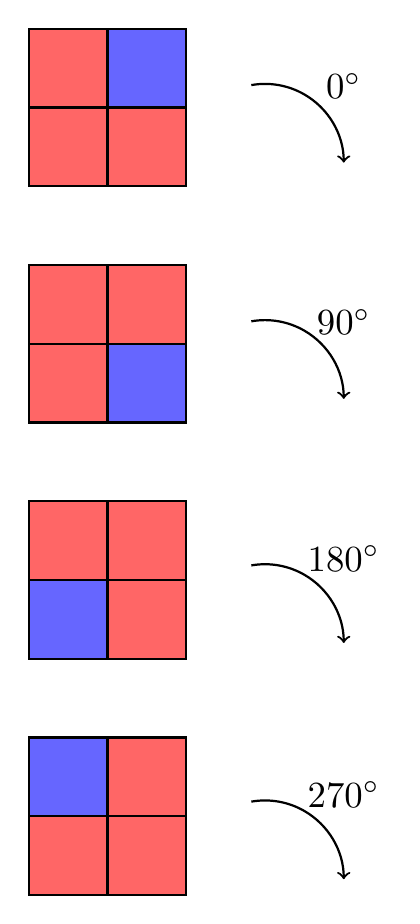
\begin{tikzpicture}

\filldraw[red!60, draw=black, thick] (-2,4) rectangle (-1,5);
\filldraw[red!60, draw=black, thick] (-2,5) rectangle (-1,6);
\filldraw[blue!60, draw=black, thick] (-1,5) rectangle (0,6);
\filldraw[red!60, draw=black, thick] (-1,4) rectangle (0,5);
\draw[thick, <-] (2,4.3) arc (0:100:1cm);
\draw (2,5.6) node[anchor=north, scale=1.33] {0$^{\circ}$};

\filldraw[red!60, draw=black, thick] (-2,1) rectangle (-1,2);
\filldraw[red!60, draw=black, thick] (-2,2) rectangle (-1,3);
\filldraw[red!60, draw=black, thick] (-1,2) rectangle (0,3);
\filldraw[blue!60, draw=black, thick] (-1,1) rectangle (0,2);
\draw[thick, <-] (2,1.3) arc (0:100:1cm);
\draw (2,2.6) node[anchor=north, scale=1.33] {90$^{\circ}$};

\filldraw[blue!60, draw=black, thick] (-2,-2) rectangle (-1,-1);
\filldraw[red!60, draw=black, thick] (-2,-1) rectangle (-1,0);
\filldraw[red!60, draw=black, thick] (-1,-1) rectangle (0,0);
\filldraw[red!60, draw=black, thick] (-1,-2) rectangle (0,-1);
\draw[thick, <-] (2,-1.8) arc (0:100:1cm);
\draw (2,-0.4) node[anchor=north, scale=1.33] {180$^{\circ}$};

\filldraw[red!60, draw=black, thick] (-2,-5) rectangle (-1,-4);
\filldraw[blue!60, draw=black, thick] (-2,-4) rectangle (-1,-3);
\filldraw[red!60, draw=black, thick] (-1,-4) rectangle (0,-3);
\filldraw[red!60, draw=black, thick] (-1,-5) rectangle (0,-4);
\draw[thick, <-] (2,-4.8) arc (0:100:1cm);
\draw (2,-3.4) node[anchor=north, scale=1.33] {270$^{\circ}$};

\end{tikzpicture}

\end{document}